\section{Integration}
\label{app:Integration}

\subsection{Coordinate Changes}

\begin{figure}[!ht]
\begin{center}
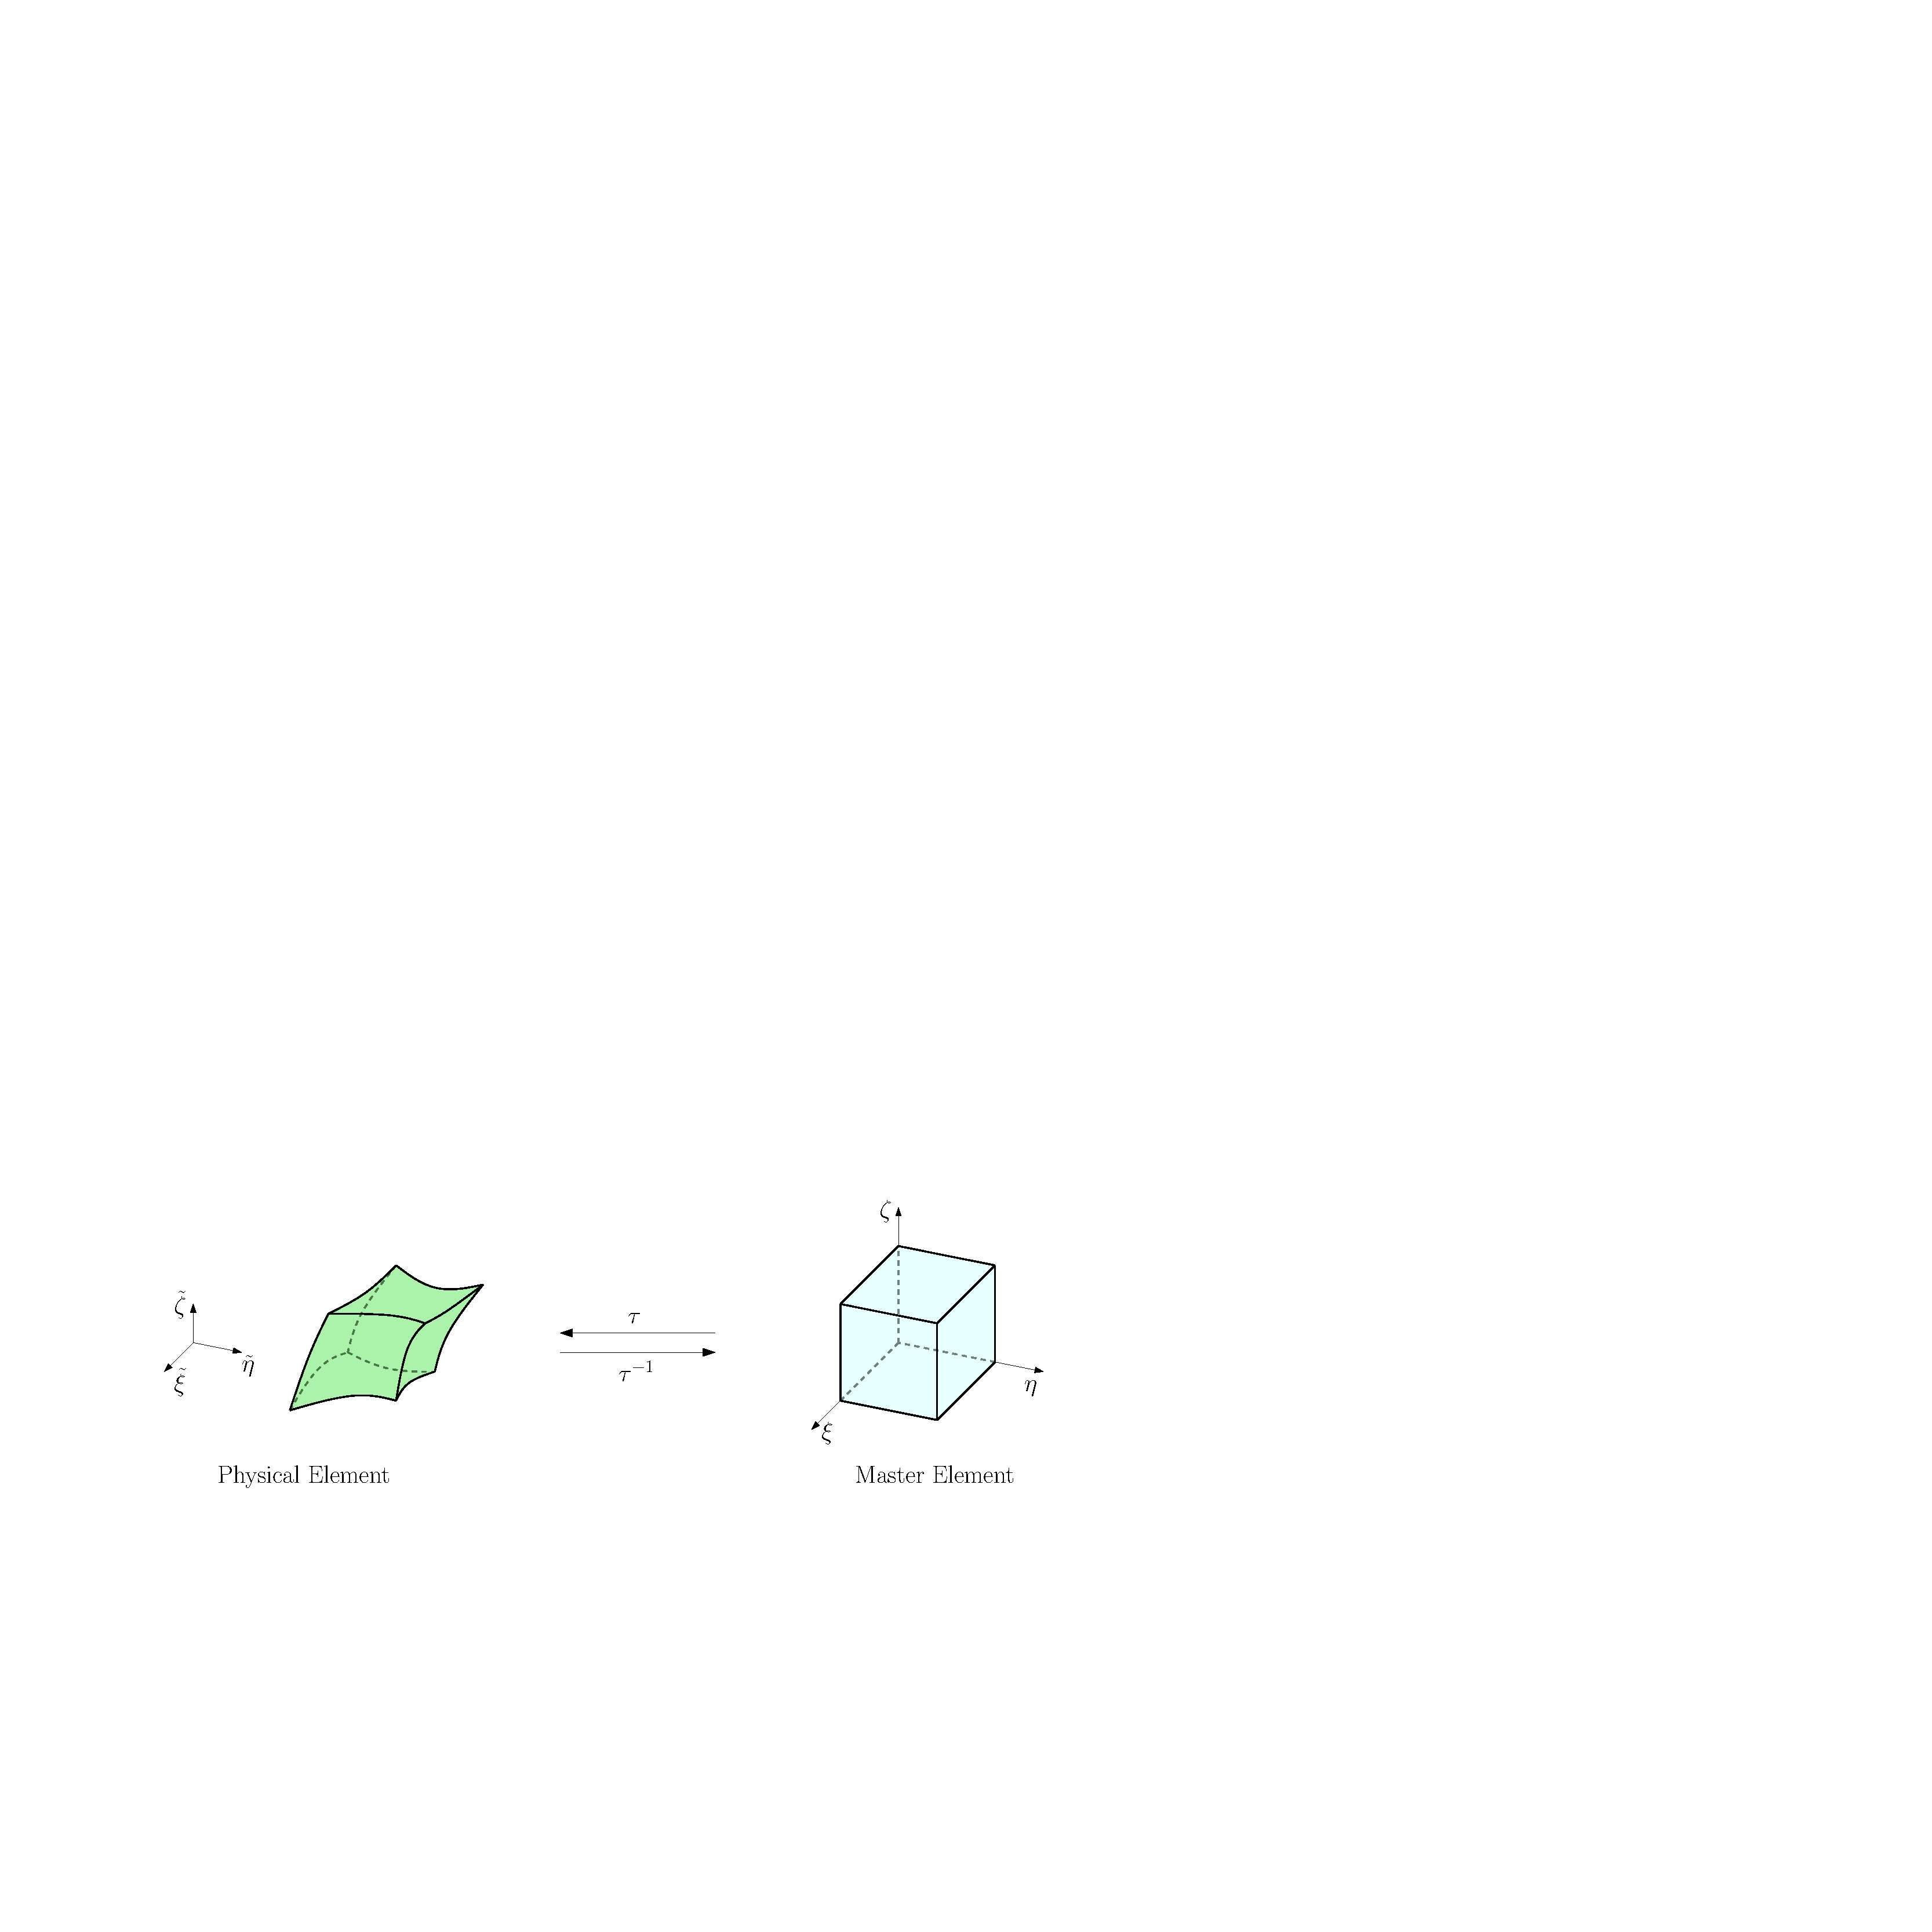
\includegraphics[scale=0.45]{./figures/CurvilinearTransform.pdf}
\caption{Transformation from the master element to the physical element.}\label{fig:curvilineartransform}
\end{center}
\end{figure}

At its core, the finite element method advocates carrying out integration over a master element domain instead of the original physical element.
It makes the method very feasible from a computational standpoint.
This involves a change of variables $\tau:\Omega\rightarrow\tilde{\Omega}$, from the master element domain $\Omega$ to the physical domain $\tilde{\Omega}$, which is assumed to be known.
This is illustrated in Figure \ref{fig:curvilineartransform}.
Note the change of variables $\tau$ is in general a nonlinear mapping.

Indeed, consider a ``physical'' integrand $f$ which is a function of variables in the different energy spaces and their differential form.
These variables are in the physical system of coordinates.
For instance, take $\phi_{\tilde{\Omega}}$, $E_{\tilde{\Omega}}$, $V_{\tilde{\Omega}}$ and $\psi_{\tilde{\Omega}}$ to represent variables in $H^1$, $H(\mathrm{curl})$, $H(\mathrm{div})$ and $L^2$ respectively.
Their corresponding differentials are $\nabla_{\tilde{\Omega}}\phi_{\tilde{\Omega}}$, $\nabla_{\tilde{\Omega}}\!\times\!E_{\tilde{\Omega}}$ and $\nabla_{\tilde{\Omega}}\!\cdot\!V_{\tilde{\Omega}}$.
However, it is their pullbacks to the master element domain, denoted with the subscript $\Omega$, which are known, since the shape functions are defined in the master element domain.\footnote{Unless the affine coordinates and their gradient are written in the physical system of coordinates, in which case one can simply substitute them in the expressions for the shape functions. This is due to the coordinate free nature of the shape functions.}
Making use of the appropriate pullback mapping for each of the variables as written in \eqref{eq:pullbacksgeneral}, this yields\footnote{In 2D, $\nabla_{\Omega}\!\times\!E_{\Omega}$ is in $L^2$, so the correct expression in the last line would be $\frac{1}{\det(J_\tau)}\nabla_{\Omega}\!\times\!E_{\Omega}$ instead of the 3D expression $\frac{1}{\det(J_\tau)}J_\tau\nabla_{\Omega}\!\times\!E_{\Omega}$. In 1D, $E_{\Omega}$ and $V_{\Omega}$ do not even exist, so they would be ignored throughout.}
\begin{equation}
	\begin{aligned}
		\mathcal{I}_{\tilde{\Omega}}&\!=\!\int_{\tilde{\Omega}}\!
			f\Big(\phi_{\tilde{\Omega}},\nabla_{\tilde{\Omega}}\phi_{\tilde{\Omega}},
				E_{\tilde{\Omega}},\nabla_{\tilde{\Omega}}\!\times\!E_{\tilde{\Omega}}, 
					V_{\tilde{\Omega}},\nabla_{\tilde{\Omega}}\!\cdot\!V_{\tilde{\Omega}}, \psi_{\tilde{\Omega}}\Big)\mathrm{d}\tilde{\Omega}\\
			&\!=\!\int_{\Omega}\!f\Big(\phi_{\tilde{\Omega}}\circ\tau, (\nabla_{\tilde{\Omega}}\phi_{\tilde{\Omega}})\circ\tau,
				E_{\tilde{\Omega}}\circ\tau,(\nabla_{\tilde{\Omega}}\!\times\!E_{\tilde{\Omega}})\circ\tau, 
					V_{\tilde{\Omega}}\circ\tau,(\nabla_{\tilde{\Omega}}\!\cdot\!V_{\tilde{\Omega}})\circ\tau,
						\psi_{\tilde{\Omega}}\circ\tau\Big)\!\det(J_\tau)\mathrm{d}\Omega\\
			&\!=\!\int_{\Omega}\!f\Big(\phi_{\Omega},J_\tau^{-\T}\nabla_{\Omega}\phi_{\Omega},
				J_\tau^{-\T}E_{\Omega},\textstyle{\frac{1}{\det(J_\tau)}}J_\tau\nabla_{\Omega}\!\times\!E_{\Omega},\\
					&\qquad\qquad\qquad\qquad\qquad\qquad\qquad\qquad\quad
						\textstyle{\frac{1}{\det(J_\tau)}}J_\tau V_{\Omega},\textstyle{\frac{1}{\det(J_\tau)}}\nabla_{\Omega}\!\cdot\!V_{\Omega},
							\textstyle{\frac{1}{\det(J_\tau)}}\psi_{\Omega}\Big)\!\det(J_\tau)\mathrm{d}\Omega\,,
	\end{aligned}
	\label{eq:integraluptomaster}
\end{equation}
where $J_\tau$ is the Jacobian matrix of the transformation $\tau:\Omega\rightarrow\tilde{\Omega}$.

Now, the integration is at least in a well known master element domain.
However, this is still a ``difficult'' domain over which to integrate (with the exception of the 1D segment, the 2D quadrilateral and the 3D hexahedron).
Hence, it is desirable to make one further change of coordinates to a ``nicer'' integration domain.
This is denoted by $\tau_Q:Q\rightarrow\Omega$, where $Q=(0,1)$ in 1D, $Q=(0,1)^2$ in 2D and $Q=(0,1)^3$ in 3D.
The transformations for each element are nicely depicted in Figure \ref{fig:integrationtransforms}. 
Some readers may have a strong preference for the integration domains $\tilde{Q}=(-1,1)$ in 1D, $\tilde{Q}=(-1,1)^2$ in 2D and $\tilde{Q}=(-1,1)^3$ in 3D.
If that is the case, then simply make the substitutions $x=\frac{\tilde{x}+1}{2}$, $y=\frac{\tilde{y}+1}{2}$ and $z=\frac{\tilde{z}+1}{2}$ in those expressions shown in Figure \ref{fig:integrationtransforms}.

%Variational methods require of integrating a function over a physical spatial domain.
%In particular the finite element method separates the domain into elements which are tranformed to the same basic set of master elements

\begin{figure}[!ht]
\begin{center}
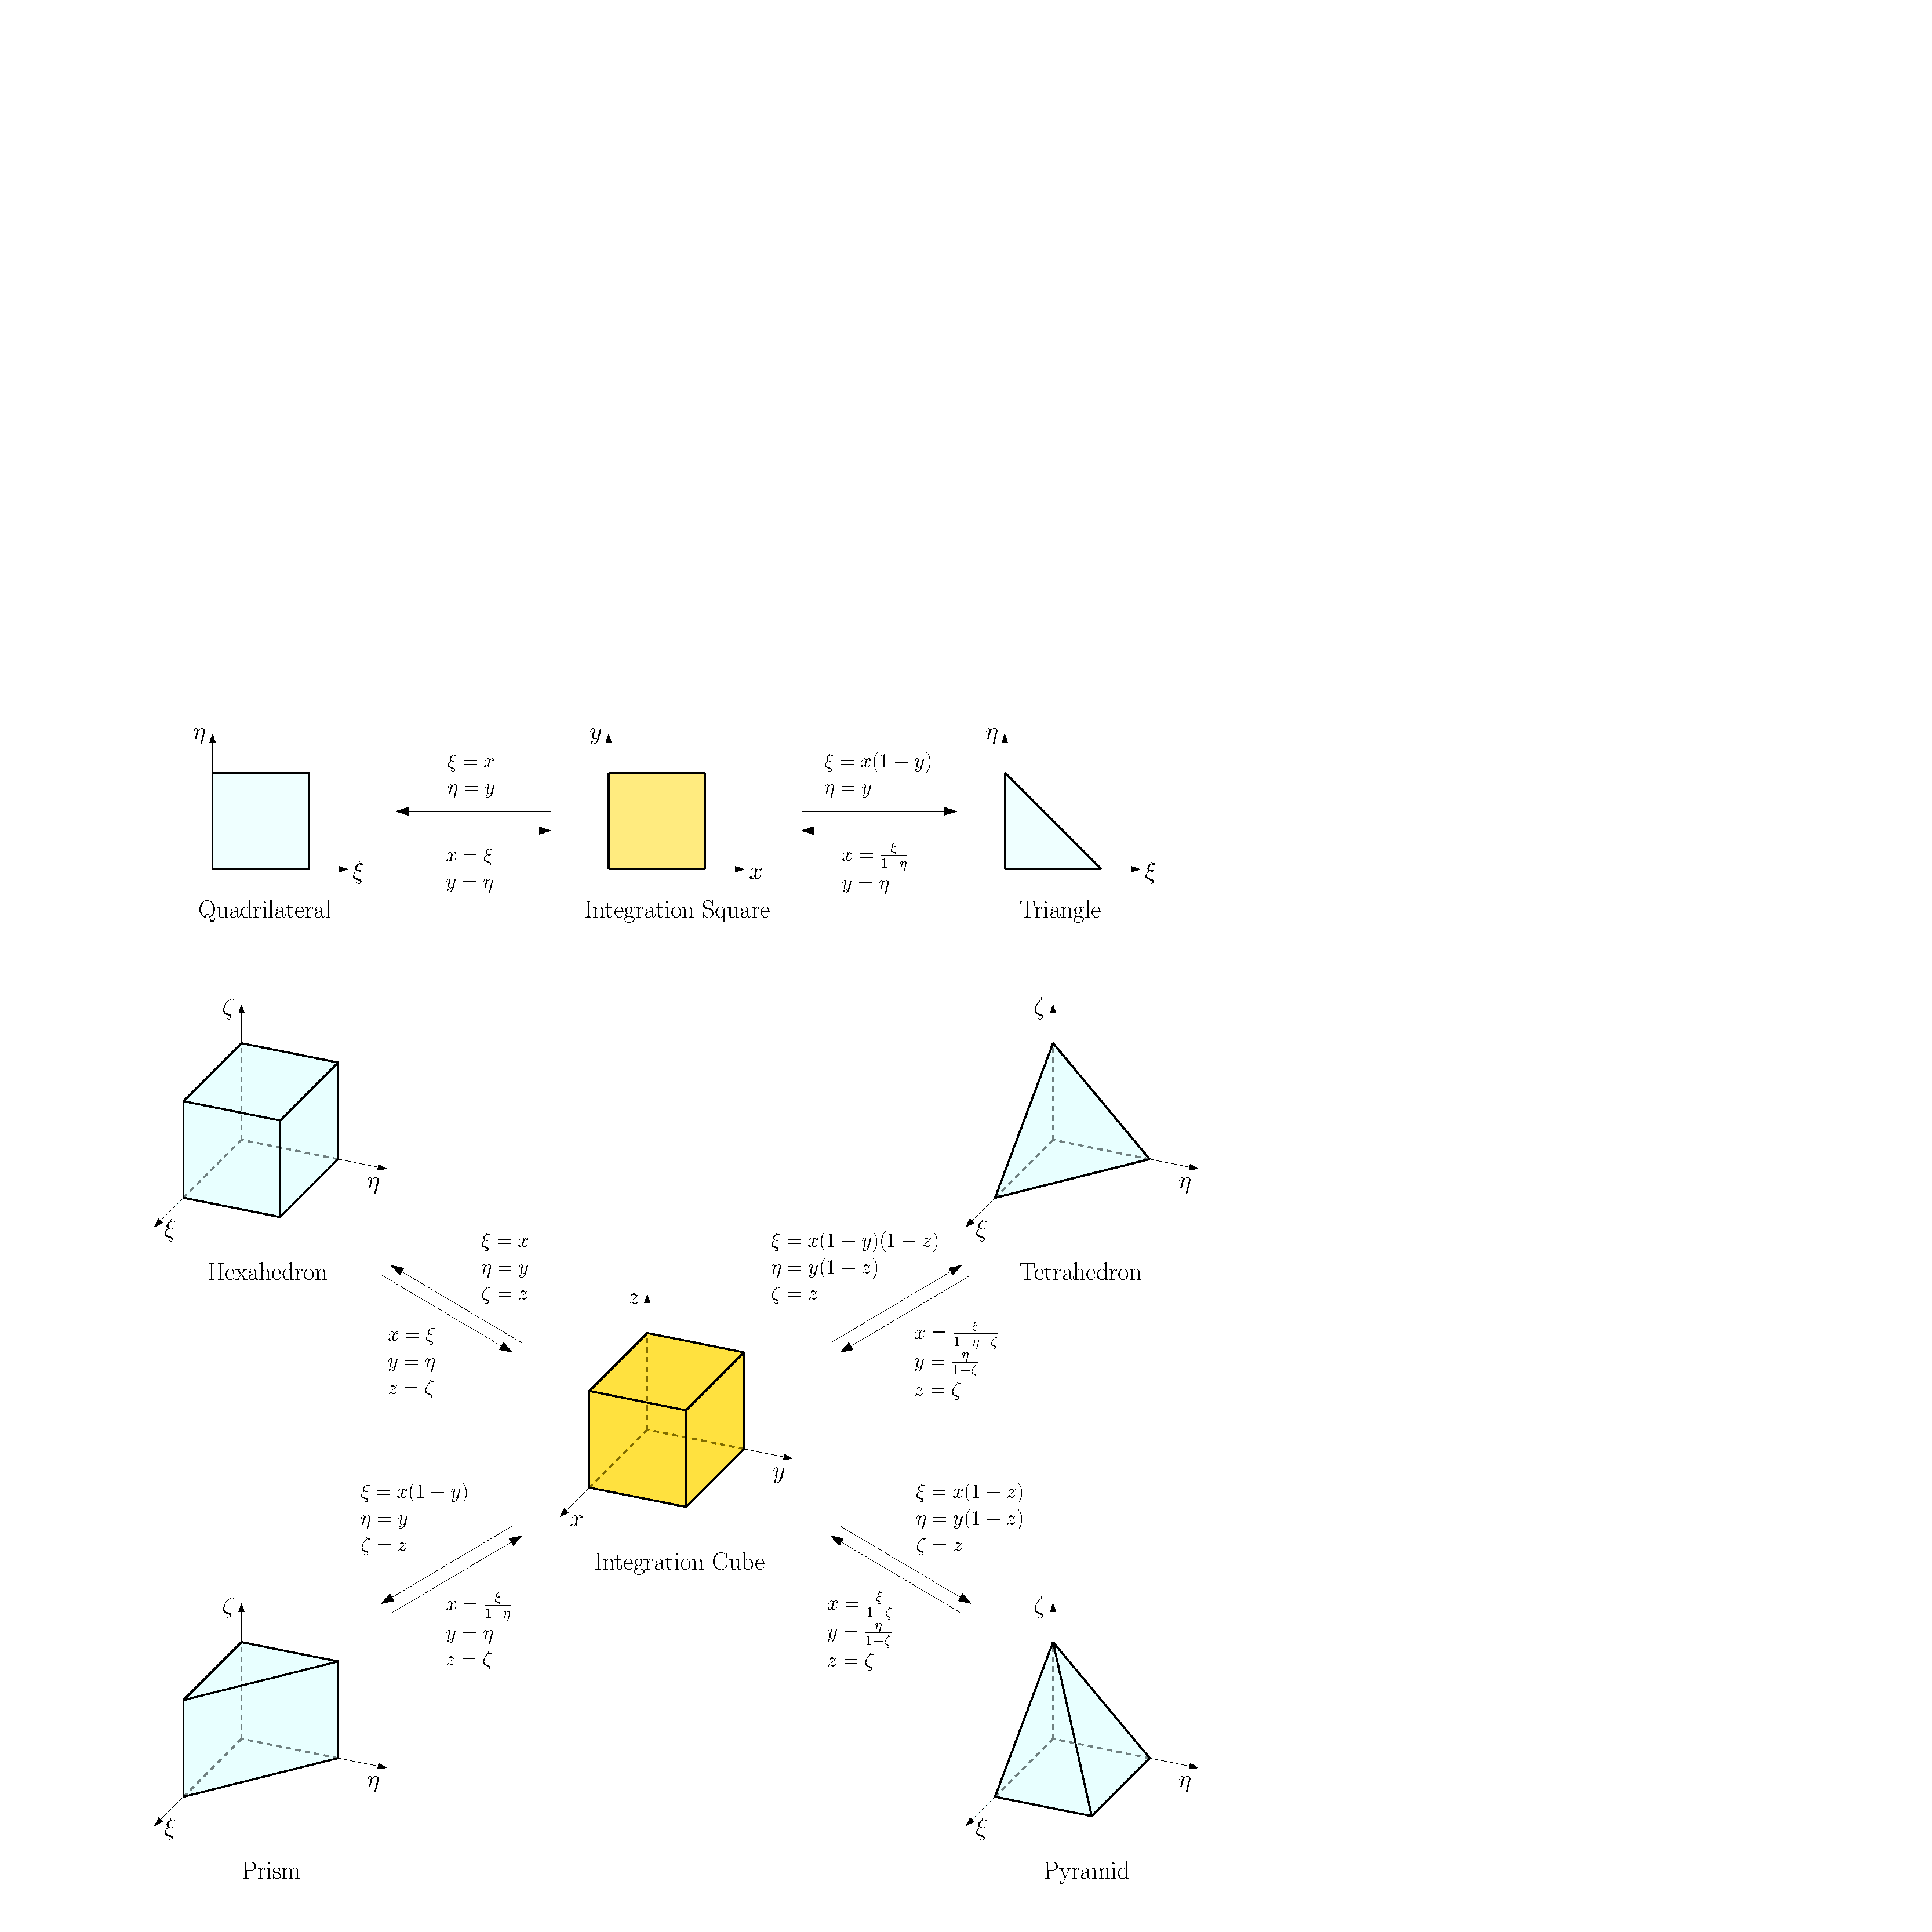
\includegraphics[scale=0.45]{./figures/IntegrationTransformations.pdf}
\caption{Transformations from each element to a nice integration domain.}\label{fig:integrationtransforms}
\end{center}
\end{figure}

%The finite element method requires integrating a function over the domain. 
%Computing these integrals over each element is therefore a fundamental step.
%Unfortunately, some elements do not have nice shapes, so it is convenient to transform them to a domain where integration is simpler to perform.
%The simplest of such domains is a square in 2D and a cube in 3D.
%Indeed, it is possible to tranform from each element to an integration square or cube as evidenced in Figure \ref{fig:integrationtransforms}.
%Note the transformations (except for the hexahedron) are nonlinear. 

The original integral in \eqref{eq:integraluptomaster} finally becomes
\begin{equation}
	\begin{aligned}
		\mathcal{I}_{\tilde{\Omega}}
			&\!=\!\int_{Q}\!f\Big(\phi_{\Omega}\circ\tau_Q,(J_\tau^{-\T}\nabla_{\Omega}\phi_{\Omega})\circ\tau_Q,
				(J_\tau^{-\T}E_{\Omega})\circ\tau_Q,(\textstyle{\frac{1}{\det(J_\tau)}}J_\tau\nabla_{\Omega}\!\times\!E_{\Omega})\circ\tau_Q,\\
					&\qquad\qquad
						(\textstyle{\frac{1}{\det(J_\tau)}}J_\tau V_{\Omega})\circ\tau_Q,
							(\textstyle{\frac{1}{\det(J_\tau)}}\nabla_{\Omega}\!\cdot\!V_{\Omega})\circ\tau_Q,
								(\textstyle{\frac{1}{\det(J_\tau)}}\psi_{\Omega})\circ\tau_Q\Big)\!\det(J_{\tau_Q})\det(J_\tau)\mathrm{d}Q\,,
	\end{aligned}
	\label{eq:integraluptoQ}
\end{equation}
where $J_{\tau_Q}$ is the Jacobian matrix of the transformation $\tau_Q:Q\rightarrow\Omega$.

\subsection{Fast integration}

To actually calculate the integral, the typical approach is to use Gaussian quadrature.
In $Q$ (or $\tilde{Q}$) the quadrature points and weights are well known and taken from the literature, and this is part of the reason why integration over the physical domain was reduced to integration over $Q$ in \eqref{eq:integraluptoQ}.

However, as the number of spatial dimensions $N$ increases from 1D to 3D, the cost grows quickly with $p$.
Indeed, to construct a typical finite element stiffness matrix, integrals usually reduce to the form
\begin{equation*}
	\mathcal{I}_{\tilde{\Omega}}=\int_{Q}u_Iv_J\mathrm{d}Q\,,
\end{equation*}
where $I=1,\ldots,\mathcal{O}(p^N)$ and $J=1,\ldots,\mathcal{O}(p^N)$.
The cost to integrate each term is $\mathcal{O}(p^N)$ as well, because there are $p+1$ quadrature points in each spatial dimension.
Hence, with a straightforward implementation, the cost to integrate all terms is $\mathcal{O}(p^{3N})$, so it is $\mathcal{O}(p^3)$ in 1D, $\mathcal{O}(p^6)$ in 2D and $\mathcal{O}(p^9)$ in 3D.
This constitutes a problem for $N\geq2$ and high $p$, so it is highly desirable to improve the integration cost.

Fortunately, the integration cost can be reduced if there exists a decoupling of either $u_I$ or $v_J$ in $x$, $y$ and $z$ (the variables after transforming to $Q$, not necessarily the variables of the physical or master element domain). 
Assume the decoupling is in $v_J$, where it takes the form $v_J(x,y)=v_{j_x}^x(x,y)v_{j_y}^y(y)$ in 2D and $v_J(x,y,z)=v_{j_x}^x(x,y,z)v_{j_y}^y(y,z)v_{j_z}^z(z)$ in 3D, with $j_x,j_y,j_z=1,\ldots,\mathcal{O}(p)$. 
Then, by reorganizing the operations and storing some coefficients, the cost is reduced to $\mathcal{O}(p^5)$ in 2D, and to $\mathcal{O}(p^7)$ in 3D.
Some of the details are in \citet{hpbook2}.
With the shape functions presented in this text, regardless of the element shape and the the associated topological entity, such a decoupling is to be expected, so this acceleration to $\mathcal{O}(p^{2N+1})$ is possible.
This technique based on a tensor product decoupling is typically called \textit{fast quadrature}.

Naturally, there are other fast integration techniques different from the fast quadrature described above which might also be applicable, but further research is required.
